%!TEX root = ../master.tex
\chapter{Evaluation}\label{ch:evaluation}
This chapter will explain how the setup for the test give a description of the setup, the procedure of the interview and results of the evaluation of the final prototype. 

\begin{figure}[!h] 
\centering
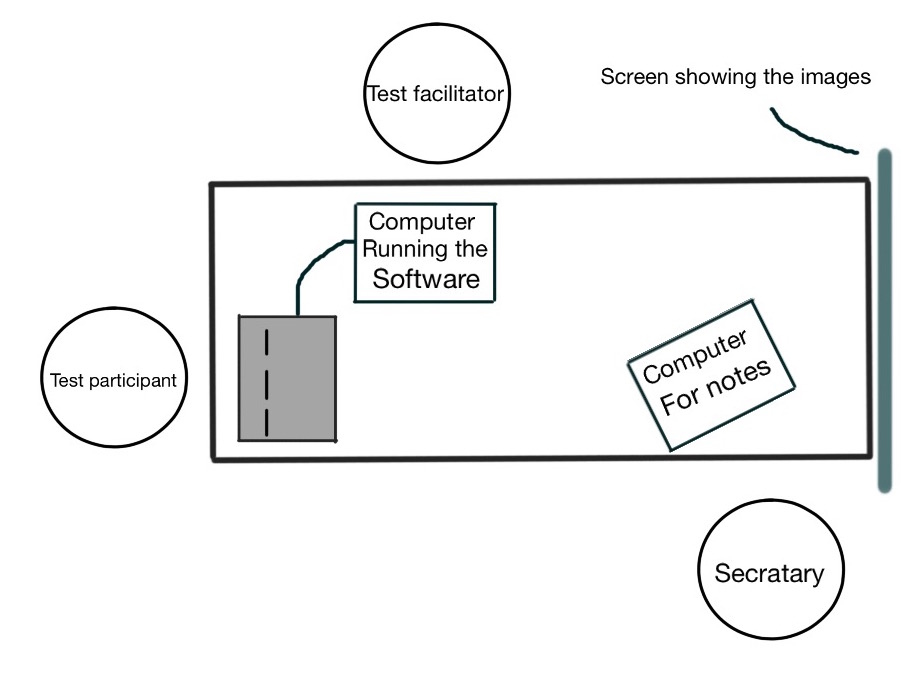
\includegraphics[width=1\textwidth]{testsetup}
\caption{\label{fig:testsetup} The test setup.}
\end{figure}

The final test was conducted on 15 test participants from Aalborg University. The participants consisted of 14 students from Medialogy and one student from Art \& Technology. The test took place in a small secluded room located at Rendsburggade 14. It was conducted by a test facilitator who interviewed the participants and instructed them in the various tasks they had to do, while observing the software performed optimally. While the testing was being conducted, a secretary took notes of what the participants answered to the question as well as how they interacted with the product.
As seen on figure \ref{fig:testsetup}, the test participant was placed in front of the product with view to a TV screen that showed the image that is being audiolised. The two images that were audiolised was the 'Mona Lisa', as can be seen in Figure \ref{fig:monalisa}, and the a painting made by Asger Jorn called 'Trolden og Fuglene' as can be seen in Figure \ref{fig:asger}. The first image to be audiolised was the 'Mona Lisa' and the second one was 'Trolden of Fuglene'. Since the software and the image that was shown on the TV screen are independent of one another, the test facilitator had to change to the corresponding on the TV screen whenever a new image was audiolised.

\begin{figure}[!h] 
\centering
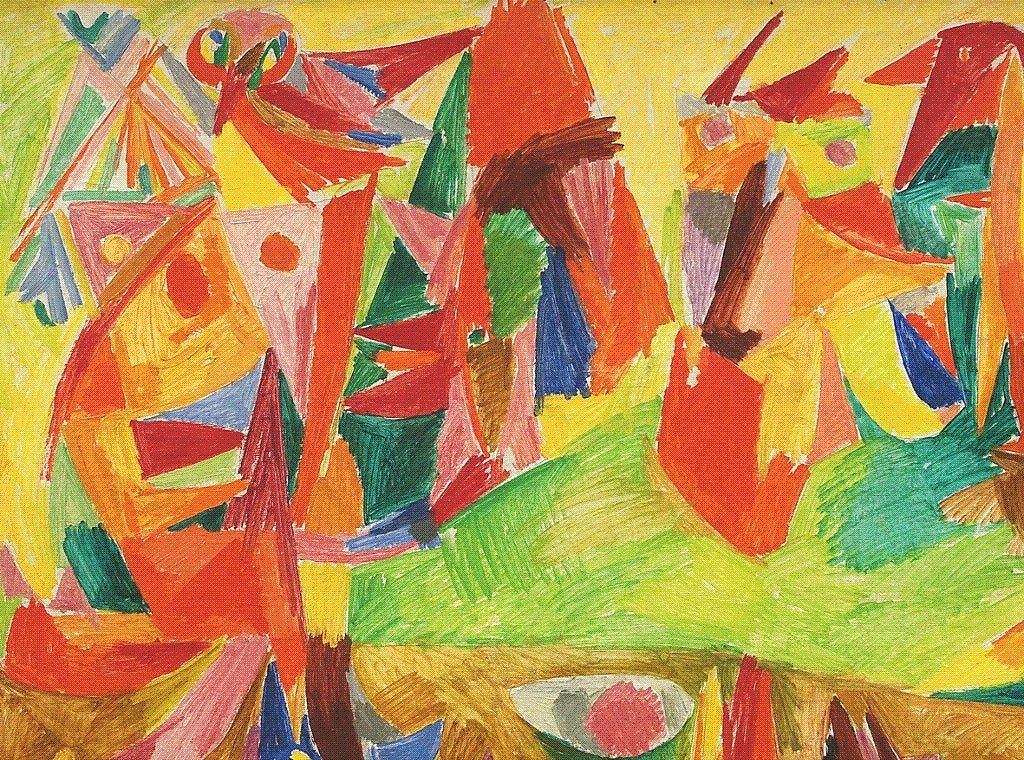
\includegraphics[width=1\textwidth]{asger}
\caption{\label{fig:asger} Asger Jorns 'Trolden og Fuglene' 1944.}
\end{figure}

\begin{figure}[!h] 
\centering
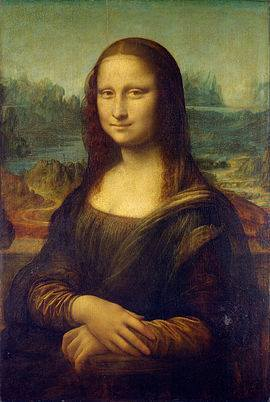
\includegraphics[width=0.5\textwidth]{monalisa}
\caption{\label{fig:monalisa} Leonardo Da Vinci 'Mona Lisa' 1503-1517.}
\end{figure}

The test was carried out by welcoming the test participant he/she was asked to sign a consent form. The test facilitator started the test by introducing the overall project and explaining what the participant was expected to do during the test such as thinking out loud (the full script can be seen in Appendix \ref{ch:appAlabel}). The test participant was first asked about the interface and what they immediately though they had to do when they saw the interface. After the test participants gave their answer, the test facilitator turned on the audiolisation of 'Mona Lisa' and told the participant to play around with the sliders. The next questions was about the audio of the product; whether the participants could hear a difference between 'MIN' and 'MAX' as well as the difference between the individual filters. Before the audiolisation changed to 'Trolden og Fuglene', the participants were asked if the text on the interface helped them understand the product better. 
After changing to the audiolisation of 'Trolden og Fuglene' the participants were asked if they could hear a difference between the two images, and again, a difference between 'MIN' and 'MAX' and a difference between the individual filters. Lastly the participants were asked to give their final thoughts.

\section{Evaluation results}


Comb filter results

\begin{table}[!h]
\centering
\caption{}
\label{tab:comb}
\begin{tabular}{|l|c|c|c|c|c|c|c|c|c|c|c|c|c|c|c|c|c|}
\hline
\multicolumn{18}{|c|}{Can you hear the difference between the "MIN" and "MAX" on the Comb filter?} \\ \hline
\multicolumn{2}{|l|}{} & \multicolumn{15}{c|}{Amount of participants} & \textbf{Total} \\ \hline
\multirow{2}{*}{\begin{tabular}[c]{@{}l@{}}Mona \\ Lisa\end{tabular}} & Yes &  &  &  &  &  &  &  &  &  &  &  &  & X &  &  & \textbf{1} \\ \cline{2-18} 
 & No & X & X & X & X & X & X & X & X & X & X & X & X &  & X & X & \textbf{14} \\ \hline
\multirow{2}{*}{\begin{tabular}[c]{@{}l@{}}Asgar \\ Jorn\end{tabular}} & Yes &  &  &  &  &  &  &  &  &  &  & X &  & X &  &  & \textbf{2} \\ \cline{2-18} 
 & No & X & X & X & X & X & X & X & X & X & X &  & X &  & X & X & \textbf{13} \\ \hline
\end{tabular}
\end{table}

Bandpass Results
\begin{table}[]
\centering
\caption{}
\label{tab:bandpass}
\begin{tabular}{|l|c|c|c|c|c|c|c|c|c|c|c|c|c|c|c|c|c|}
\hline
\multicolumn{18}{|c|}{Can you hear the difference between the "MIN" and "MAX" on the Bandpass filter?} \\ \hline
\multicolumn{2}{|l|}{} & \multicolumn{15}{c|}{Amount of participants} & \textbf{Total} \\ \hline
\multirow{2}{*}{\begin{tabular}[c]{@{}l@{}}Mona \\ Lisa\end{tabular}} & Yes & X & X &  & X & X & X & X &  & X & X & X & X & X &  &  & \textbf{11} \\ \cline{2-18} 
 & No &  &  & X &  &  &  &  & X &  &  &  &  &  & X & X & \textbf{4} \\ \hline
\multirow{2}{*}{\begin{tabular}[c]{@{}l@{}}Asgar \\ Jorn\end{tabular}} & Yes & X & X & X & X & X & X & X &  & X & X & X & X & X &  & X & \textbf{13} \\ \cline{2-18} 
 & No &  &  &  &  &  &  &  & X &  &  &  &  &  & X &  & \textbf{2} \\ \hline
\end{tabular}
\end{table}


High shelf results
\begin{table}[]
\centering
\caption{}
\label{tab:highshelf}
\begin{tabular}{|l|c|c|c|c|c|c|c|c|c|c|c|c|c|c|c|c|c|}
\hline
\multicolumn{18}{|c|}{Can you hear the difference between the "MIN" and "MAX" on the High Shelf filter?} \\ \hline
\multicolumn{2}{|l|}{} & \multicolumn{15}{c|}{Amount of participants} & \textbf{Total} \\ \hline
\multirow{2}{*}{\begin{tabular}[c]{@{}l@{}}Mona \\ Lisa\end{tabular}} & Yes & X & X & X & X & X & X & X & X & X & X & X & X & X & X & X & \textbf{15} \\ \cline{2-18} 
 & No &  &  &  &  &  &  &  &  &  &  &  &  &  &  &  & \textbf{0} \\ \hline
\multirow{2}{*}{\begin{tabular}[c]{@{}l@{}}Asgar \\ Jorn\end{tabular}} & Yes & X & X & X & X & X & X & X & X & X & X & X & X & X & X & X & \textbf{15} \\ \cline{2-18} 
 & No &  &  &  &  &  &  &  &  &  &  &  &  &  &  &  & \textbf{0} \\ \hline
\end{tabular}
\end{table}

Is the "help text" useful you you?
\begin{table}[!h]
\centering
\caption{}
\label{tab:helptext}
\begin{tabular}{|l|c|c|c|c|c|c|c|c|c|c|c|c|c|c|c|c|}
\hline
\multicolumn{17}{|c|}{Is the "help text" usefull to you?} \\ \hline
 & \multicolumn{15}{c|}{Amount of participants} & \textbf{Total} \\ \hline
Yes &  & X & X & X & X & X & X & X & X & X & X & X & X & X & X & \textbf{14} \\ \hline
No & X &  &  &  &  &  &  &  &  &  &  &  &  &  &  & \textbf{1} \\ \hline
\end{tabular}
\end{table}

Can you hear a difference between the two images?
\begin{table}[!h]
\centering
\caption{}
\label{tab:twoimagedifference}
\begin{tabular}{|l|c|c|c|c|c|c|c|c|c|c|c|c|c|c|c|c|}
\hline
\multicolumn{17}{|c|}{Can you hear a difference between the two images?} \\ \hline
 & \multicolumn{15}{c|}{Amount of participants} & \textbf{Total} \\ \hline
Yes & X & X & X & X & X & X & X & X & X & X & X & X & X & X & X & \textbf{15} \\ \hline
No &  &  &  &  &  &  &  &  &  &  &  &  &  &  &  & \textbf{0} \\ \hline
\end{tabular}
\end{table}


\section{Results analysis}
This section describes the results found in the final test. The results were found by making a semi-structured interview and getting qualitative feedback by communicating directly with the user, using the script shown above. 

From the testing, 13 of the participants found it difficult to hear the difference between "MIN" and "MAX" when manipulating with the comb filter on both Mona Lisa and Asger Jorns picture. However, when using the Bandpass and High shelf, the user could hear a clear difference between the two filters when changing the values using the sliders. Two of the test participants had no clear comments regarding the difference between any of the filters. These answers was marked as "not clear for use" in case the test facilitator and secretary had misunderstood the participant's answer. 

Nine of the participants did not know the terms of the different filters, but they could distinguish a change in the output when manipulating with the sliders. Therefore, they did not know exactly what to listen for when manipulating with the sliders. Six of the participants from Medialogy knew the terms of the three filters. Even though six of the participants knew the terms of the filters, only two knew exactly what the filters did, and what they had to listen for when manipulating with the sliders. 

The interface was clear for all the participants and they knew how to use it, either by looking at the help text or at the sliders. None of the test participants had any trouble manipulating with the sliders. 

All of the participants could hear a clear difference between the colourful Asger Jorn painting and the darker Mona Lisa painting. They all suspected the difference in the colours for being the reason for the difference in the sound. 

To sum up the overall thoughts on the product, the test participants found the device to be very easy to use, even though most of them did not know what the filters actually did or what the names of the filters meant. 

\todo {One particpant was asking if the later iteration would show the context between the picture and sound to find a balanced and satisfying output}. 